
%%%%%%%%%%%%%%%%%%%%%%%%%%%%%%%%%%%%%%%%%%%%%%%%%%%%%%%%%%%%%%%%%%%%%%%%%%%%%%%%%%%%%%%%%%%%%%%%%%%%%%%%%%%%%%%%%%% problem

\section{Problem For High Level Synthesis}

From this section till the end of this paper we will consider that the specification for high level synthesis is already specified through:

\begin{itemize}
\item Sequencing Graph
\item Set of functional resources
\item Set of constraint
\end{itemize}

After we have the specification, we are ready for synthesis process. This is where various of problem arise. To make the problem and solution unity and easy to be understood, I will explain base on only one main equation. 

consider the equation \ref{main}, we can break it into a a few iteration and each iteration consist of equations \ref{1} ,\ref{2},\ref{3} and \ref{4}. Sequencing graph for each iteration is shown in figure \ref{fig:Scheduled_sequencing_graph}

\begin{equation}\label{main}
 y'' = 3xy'+ 3y =0
\end{equation}

\begin{equation}\label{1}
 x1=x+dx
\end{equation}
\begin{equation}\label{2}
u1 = u -(3*x*u*dx)-(3*y*dx)
\end{equation}
\begin{equation}\label{3}
 y1 =y+(u*dx)
\end{equation}
\begin{equation}\label{4}
 c = x1<a
\end{equation}


\begin{figure}[h]
    \centering
    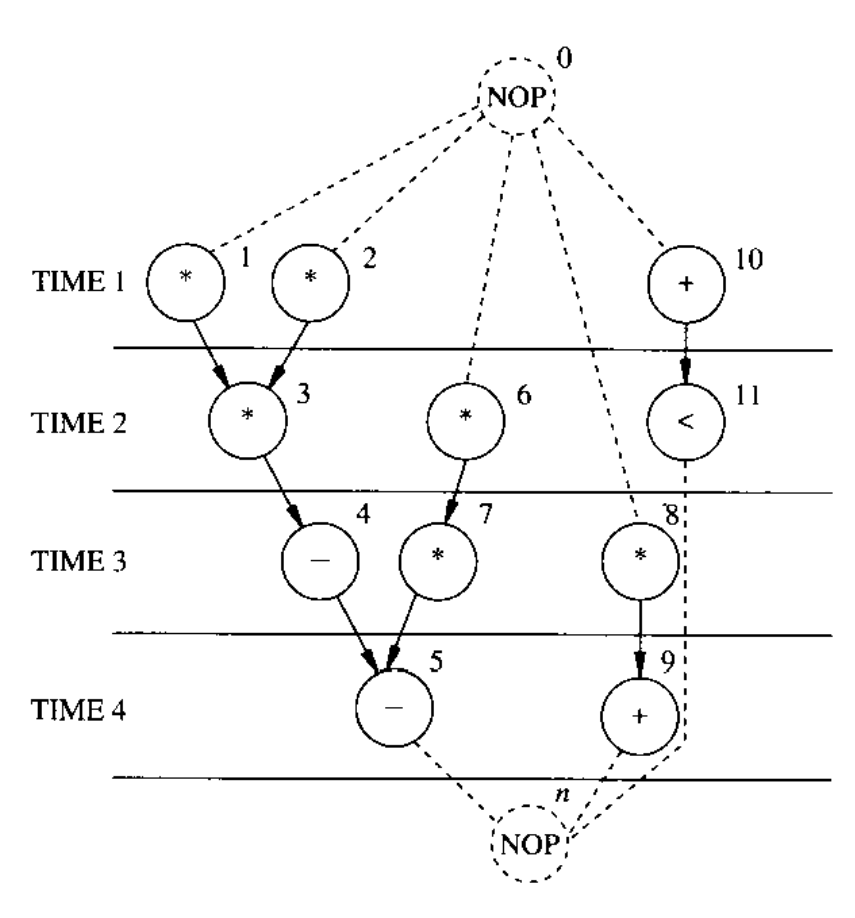
\includegraphics[width=0.5\textwidth]{scheduled_sequencing_graph}
    \caption{ Scheduled sequencing graph \cite{b1}}
    \label{fig:Scheduled_sequencing_graph}
\end{figure}

from now on we will use this graph as our main reference. 

\subsection{Functional Resource Sharing and Binding problem}

Base on figure \ref{fig:Scheduled_sequencing_graph}, we need atleast 11 resource to cover all operation. But this direct solution cause many implication like large used area and cost inefficient. For that reasons some operation need to share the same resources if possible as illustrated in figure \ref{fig:Scheduled_sequencing_graph_with} where the operation within bounded area share the same resource. This where binding problem arise, where we need to bind the operation to the right resource in the way that conflict can be avoided. To handle this problem we we need solve it through resource sharing and binding analysis that we will discuss in resource sharing and binding  analysis section 

\begin{figure}[h]
    \centering
    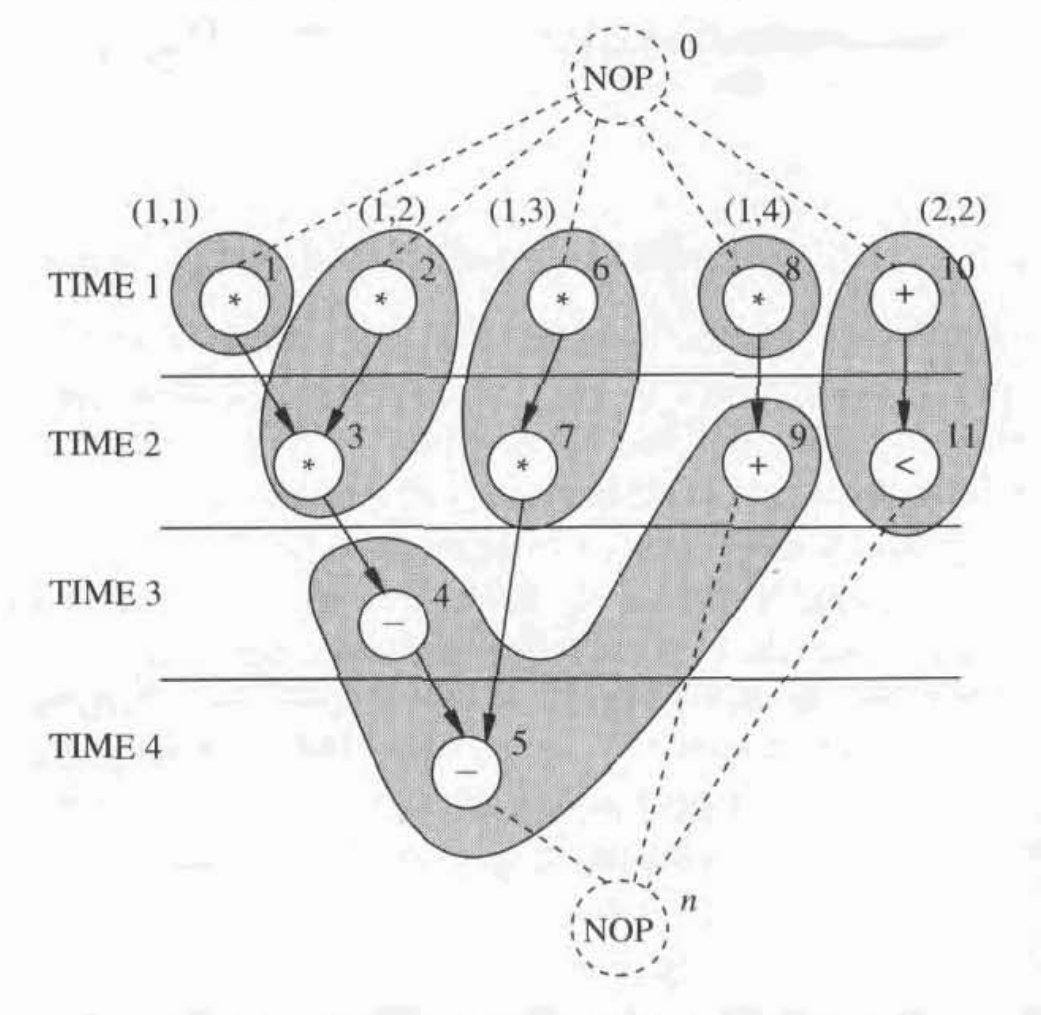
\includegraphics[width=0.4\textwidth]{Scheduled_sequencing_graph_with}
    \caption{ Scheduled sequencing graph with resource binding. \cite{b1}}
    \label{fig:Scheduled_sequencing_graph_with}
\end{figure} 


\subsection{Register Sharing problem}

Base on the figure above, there is intermediate variable that we need to store. If we choose to have one register for each variable, it cause high used area and and cost inefficient. For that reason we need to reduce the number of register. Thus, we need a solution so that the variable could share the same register. This problem will be discussed more in register sharing section.


%%%%%%%%%%%%%%%%%%%%%%%%%%%%%%%%%%%%%%%%%%%%%%%%%%%%%%%%%%%%%%%%%%%%%%%%%%%%%%%%%%%%%%%%%%%%%%%%%%%%%%%%


